\chapter{Implementacija i korisničko sučelje}

		\section{Korištene tehnologije i alati}

			 U timu smo za vrijeme projekta komunicirali ponajviše preko aplikacija Whatsapp\footnote{\url{https://www.whatsapp.com/}} te Discorda\footnote{\url{https://discord.com/}}, a sa asistentom i demonstratorom preko Microsoft Teams\footnote{\url{https://teams.microsoft.com/v2/}} i Microsoft Outlook\footnote{\url{https://outlook.office.com/mail/}}. Tekst u dokumentaciji smo uređivali pomoću latex-a\footnote{\url{https://www.latex-project.org/}} u editoru texStudio\footnote{\url{https://www.texstudio.org/}} te generirali PDF dokument iz latex dokumenta pomoću TexLive\footnote{\url{https://www.tug.org/texlive/}}. Dijagrame uporabe, sekvencijske dijagrame, dijagram razsmještaja i aktivnosti smo izradili pomoću alata Astah UML\footnote{\url{https://astah.net/products/astah-um}l/}.Dijagram razreda smo napravili pomoću VisualParadigm\footnote{\url{https://www.visual-paradigm.com/}}. Model baze podataka je napravljen pomoću alata ERDplus\footnote{\url{https://erdplus.com/}}. Kako bi smo zajedno mogli raditi na projektu u isto vrijeme te ujedno i pratiti razvojne verzije koristili smo Git\footnote{\url{https://git-scm.com/}} zajedno sa udaljenim repozitorijom GitHub\footnote{\url{https://github.com/}}. Razvojna okruženja koja su korištena su Visual Studio Code\footnote{\url{https://code.visualstudio.com/}} te pgAdmin4\footnote{\url{https://www.pgadmin.org/}}. Frontend je napisan u programskom jezika javascript\footnote{\url{https://www.javascript.com/}} pomoću biblioteke React\footnote{\url{https://react.dev/}}, dok je za backend korišten PostgreSQL\footnote{\url{https://www.postgresql.org/}}. Unit testovi su odrađeni pomoću alata pgTAP\footnote{\url{https://pgtap.org/}}, dok su integracijski testovi napravljeni pomoću alata Selenium\footnote{\url{https://www.selenium.dev/selenium-ide/}} i programskog  jezika Python\footnote{\url{https://www.python.org/}}.
			 Aplikacija je puštena u pogon na servisu render\footnote{\url{https://render.com/}}.
			\eject 
		
	
		\section{Ispitivanje programskog rješenja}
			
			\subsection{Ispitivanje komponenti}
				Ispitivanje jedinica je provedeno pomoću alata pgTAP. pgTAP je skup funkcija baze podataka koje olakšavaju pisanje testova. Pomoću ovog smo alata testirali izvođenje i ponašanje backenda-a ostvarenog kroz funkcije u bazi napisane plpgsql programskim jezikom. Alat nudi brojne definirane metode koje omogućuju definiranje očekivanog ispisa za određeni ulaz, uspoređivanje rezultata odrađene funkcije sa podacima iz tablica, itd.
				\eject
				\subsection{Ispitni slučaj 1 - funkcionalnost prijave}
				Ovaj ispitni slučaj ispituje funkcionalnost prijave u sustav. Testovi ispitnog slučaja testiraju postoji li funkcija u bazi, je li funkcija napisana plpgsql jezikom te koji su ulazni i izlazni tipovi podataka funkcije. To se testira koristeći ugrađene funkcije pgTAP-a kao što su \textit{\texttt{has\_function}} za testiranje postoji li definirana funkcija u bazi, \textit{\texttt{function\_lang\_is}} za testiranje je li funkcija napisana plpgsql jezikom, \textit{\texttt{function\_returns}} za testiranje vraća li funkcija neki tip podataka ili je tipa void, \textit{\texttt{is\(\)}} za provjeru dvaju argumenata te na osnovu njihovog podudaranje ili odudaranja se izbacuje rezultat. Rezultat je uvijek u obliku jednog reda sa jednom kolonom koja može sadržavati tekst \textit{ok $<$broj testa$>$ - $<$opis testa$>$} ili \textit{not ok $<$broj testa$>$ - $<$opis testa$>$}.
				\begin{figure}[H]
					\centering
					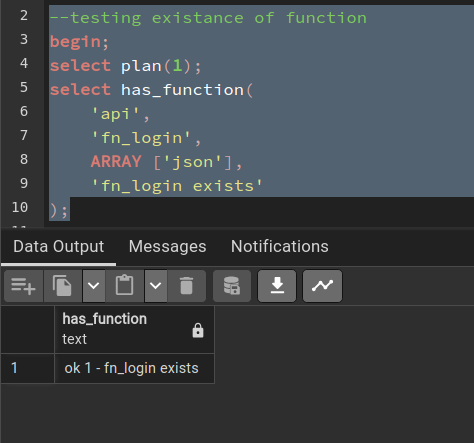
\includegraphics[width=\textwidth]{slike/unit_tests/ut_1/has_func.png}
					\caption{Pokretanje testa za provjeru postojanja funkcije}
					\label{fig: IS1-has_function}
				\end{figure}
				\begin{figure}[H]
					\centering
					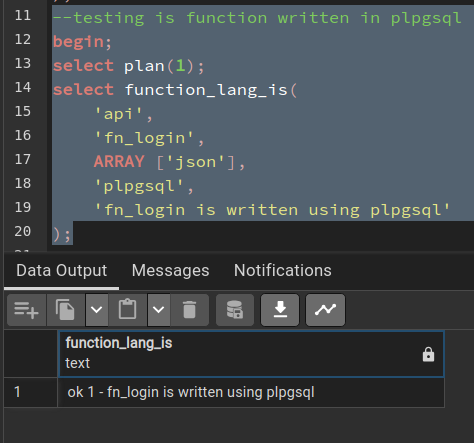
\includegraphics[width=\textwidth]{slike/unit_tests/ut_1/func_lang.png}
					\caption{Pokretanje testa za provjeru jezika kojim je napisana funkcija}
					\label{fig: IS1-function_lang}
				\end{figure}
				\begin{figure}[H]
					\centering
					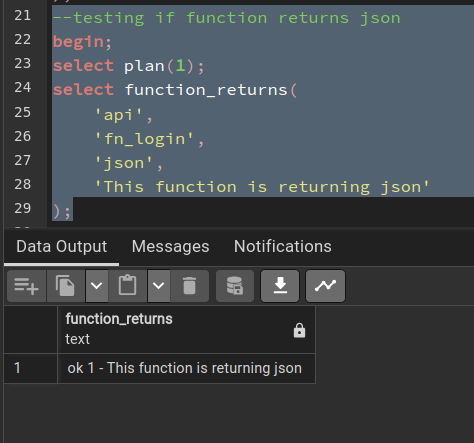
\includegraphics[width=\textwidth]{slike/unit_tests/ut_1/func_return.png}
					\caption{Pokretanje testa za provjeru povratnog tipa podatka funkcije}
					\label{fig: IS1-function_return}
				\end{figure}
				\begin{figure}[H]
					\centering
					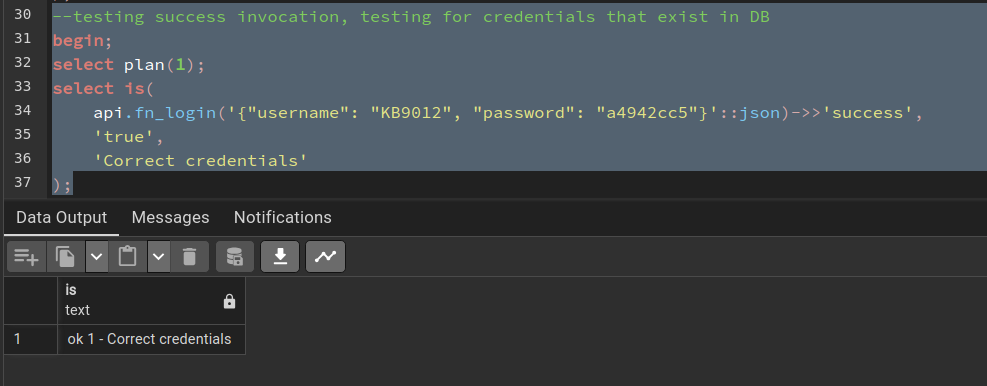
\includegraphics[width=\textwidth]{slike/unit_tests/ut_1/success_login.png}
					\caption{Pokretanje testa za provjeru rada same funkcije, uspjeh}
					\label{fig: IS1-uspješni login}
				\end{figure}
				\begin{figure}[H]
					\centering
					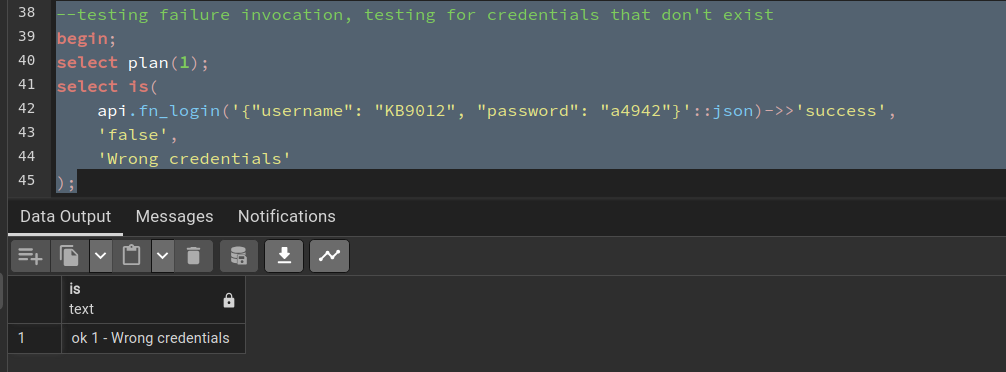
\includegraphics[width=\textwidth]{slike/unit_tests/ut_1/failure_login.png}
					\caption{Pokretanje testa za provjeru rada same funkcije, neuspjeh}
					\label{fig: IS1-neuspješni login}
				\end{figure}
				\begin{figure}[H]
					\centering
					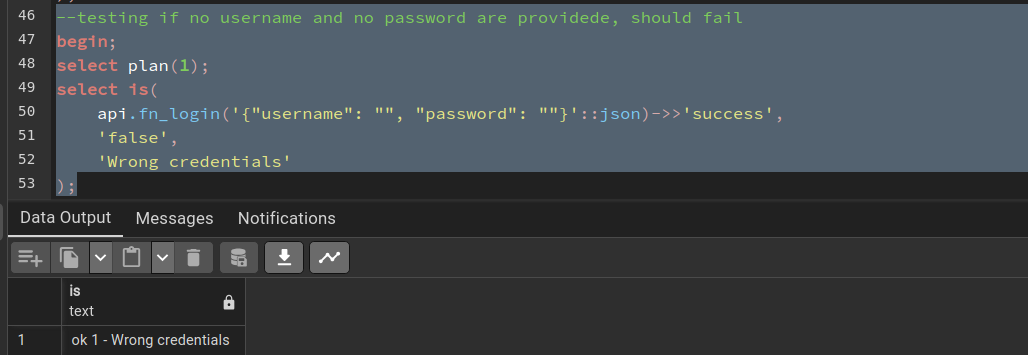
\includegraphics[width=\textwidth]{slike/unit_tests/ut_1/no_creds.png}
					\caption{Pokretanje testa za provjeru rada same funkcije, neuspjeh}
					\label{fig: IS1-login bez vjerodajnica}
				\end{figure}
				\begin{figure}[H]
					\centering
					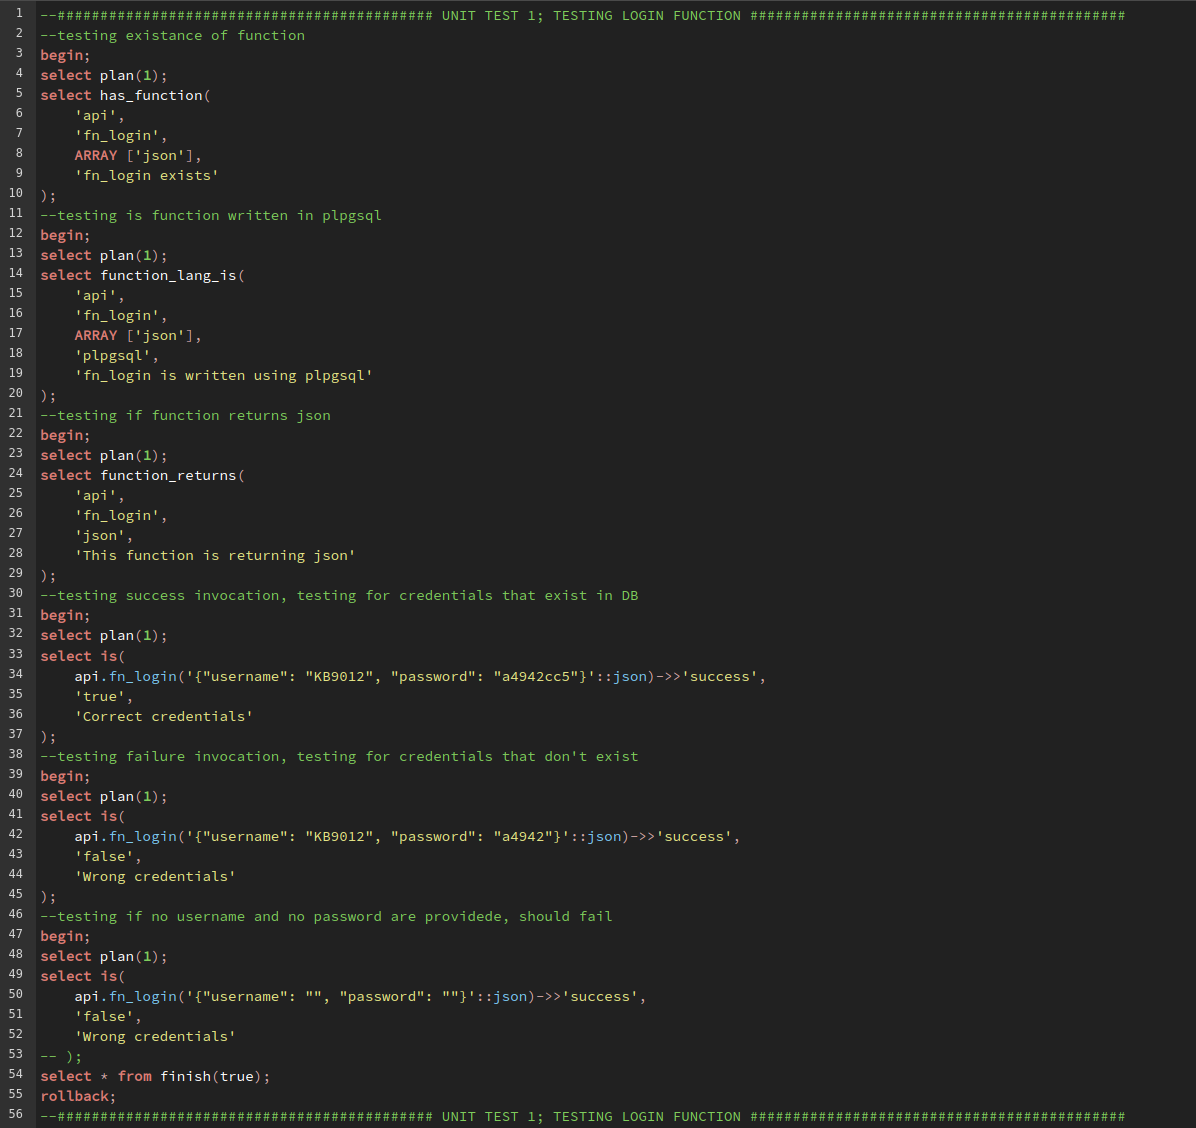
\includegraphics[width=\textwidth]{slike/unit_tests/ut_1/code.png}
					\caption{Kod ispitnog slučaja 1}
					\label{fig: IS1-kod}
				\end{figure}
				\eject
				\subsection{Ispitni slučaj 2 - funkcionalnost dodavanja novog administratora}
				Ovaj ispitni slučaj ispituje funkcionalnost dodavanja novog administratora. Testovi ispitnog slučaja testiraju postoji li funkcija u bazi, je li funkcija napisana plpgsql jezikom te koji su ulazni i izlazni tipovi podataka funkcije. To se testira koristeći ugrađene funkcije pgTAP-a kao što su \textit{\texttt{has\_function}} za testiranje postoji li definirana funkcija u bazi, \textit{\texttt{function\_lang\_is}} za testiranje je li funkcija napisana plpgsql jezikom, \textit{\texttt{function\_returns}} za testiranje vraća li funkcija neki tip podataka ili je tipa void, \textit{\texttt{is\(\)}} ze provjeru dvaju argumenata te na osnovu njihovog podudaranje ili odudaranja se izbacuje rezultat. Rezultat je uvijek u obliku jednog reda sa jednom kolonom koja može sadržavati tekst \textit{ok $<$broj testa$>$ - $<$opis testa$>$} ili \textit{not ok $<$broj testa$>$ - $<$opis testa$>$}.
				\begin{figure}[H]
					\centering
					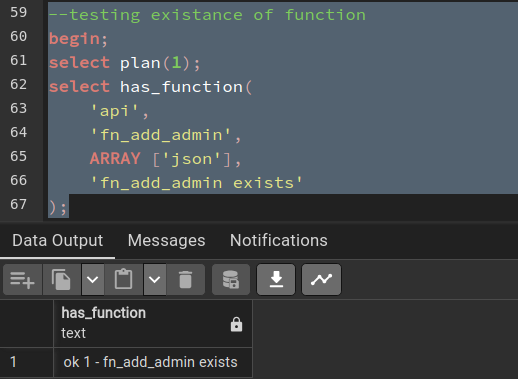
\includegraphics[width=\textwidth]{slike/unit_tests/ut_2/has_func.png}
					\caption{Pokretanje testa za provjeru postojanja funkcije}
					\label{fig: IS2-has_function}
				\end{figure}
				\begin{figure}[H]
					\centering
					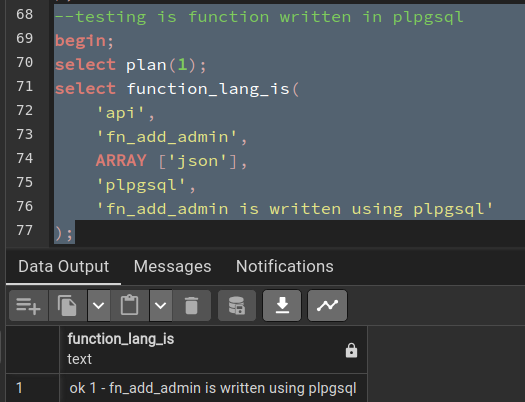
\includegraphics[width=\textwidth]{slike/unit_tests/ut_2/func_lang.png}
					\caption{Pokretanje testa za provjeru jezika kojim je napisana funkcija}
					\label{fig: IS2-function_lang}
				\end{figure}
				\begin{figure}[H]
					\centering
					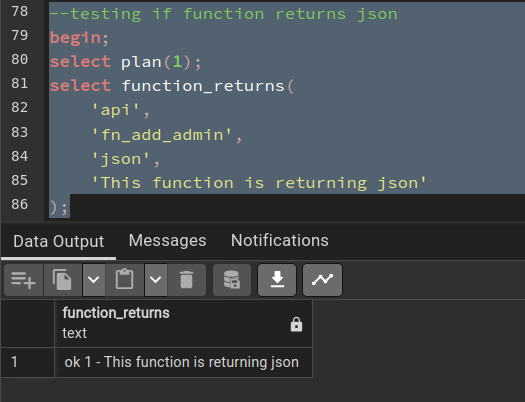
\includegraphics[width=\textwidth]{slike/unit_tests/ut_2/func_return.png}
					\caption{Pokretanje testa za provjeru povratnog tipa podatka funkcije}
					\label{fig: IS2-function_return}
				\end{figure}
				\begin{figure}[H]
					\centering
					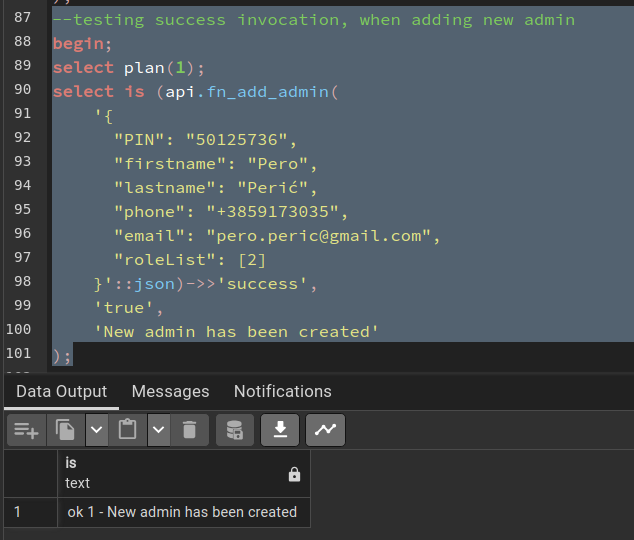
\includegraphics[width=\textwidth]{slike/unit_tests/ut_2/success_invocation.png}
					\caption{Pokretanje testa za provjeru rada same funkcije, uspjeh}
					\label{fig: IS2-uspješno kreiran administrator}
				\end{figure}
				\begin{figure}[H]
					\centering
					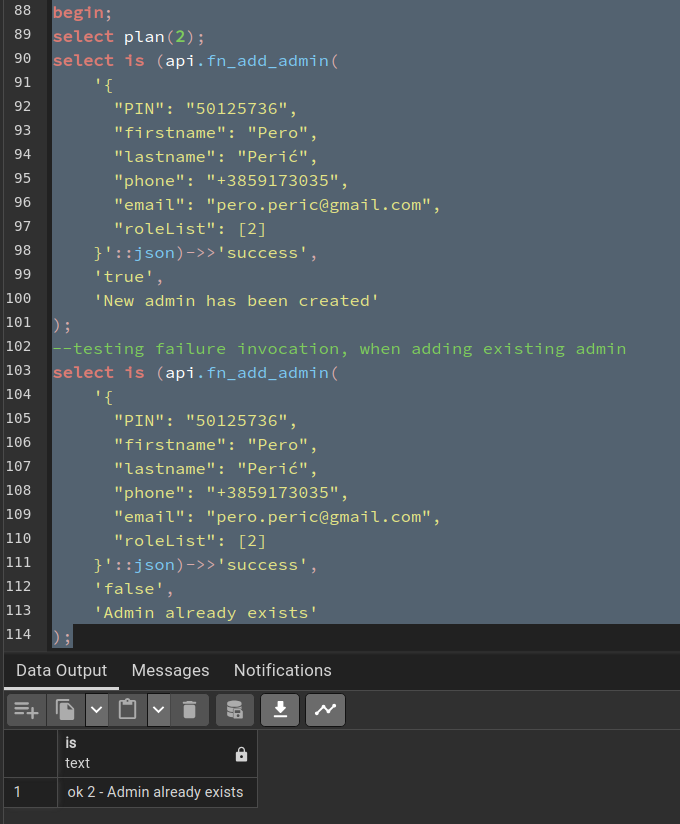
\includegraphics[width=\textwidth]{slike/unit_tests/ut_2/failure_invocation.png}
					\caption{Pokretanje testa za provjeru rada same funkcije, neuspjeh}
					\label{fig: IS2-administrator nije kreiran, već postoji isti}
				\end{figure}
				\begin{figure}[H]
					\centering
					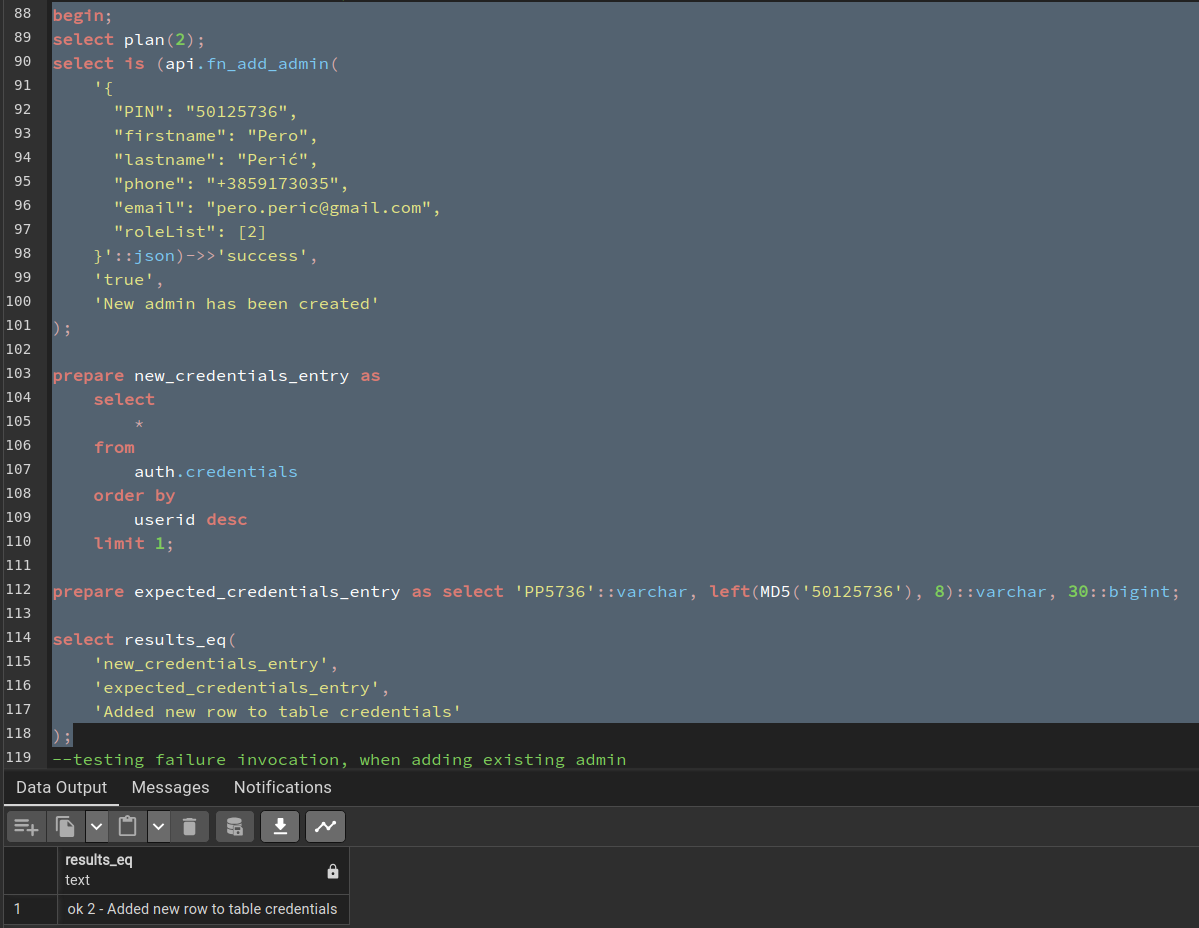
\includegraphics[width=\textwidth]{slike/unit_tests/ut_2/credentials_creation.png}
					\caption{Pokretanje testa za provjeru automatskog kreiranja vjerodajnica za novog administratora}
					\label{fig: IS2-kreirane vjerodajnice za novod administratora}
				\end{figure}
				\begin{figure}[H]
					\centering
					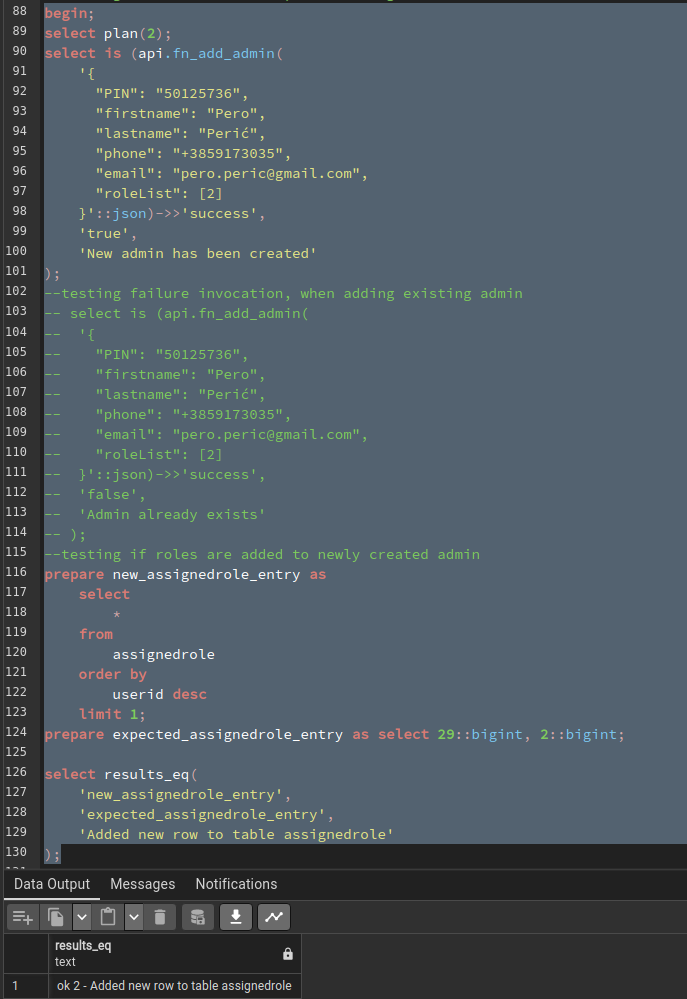
\includegraphics[width=\textwidth]{slike/unit_tests/ut_2/role_assigned.png}
					\caption{Pokretanje testa za provjeru automatskog dodjeljivanja uloge/uloga za novog administratora}
					\label{fig: IS2-dodavanje uloga novom adminstratoru}
				\end{figure}
				\begin{figure}[H]
					\centering
					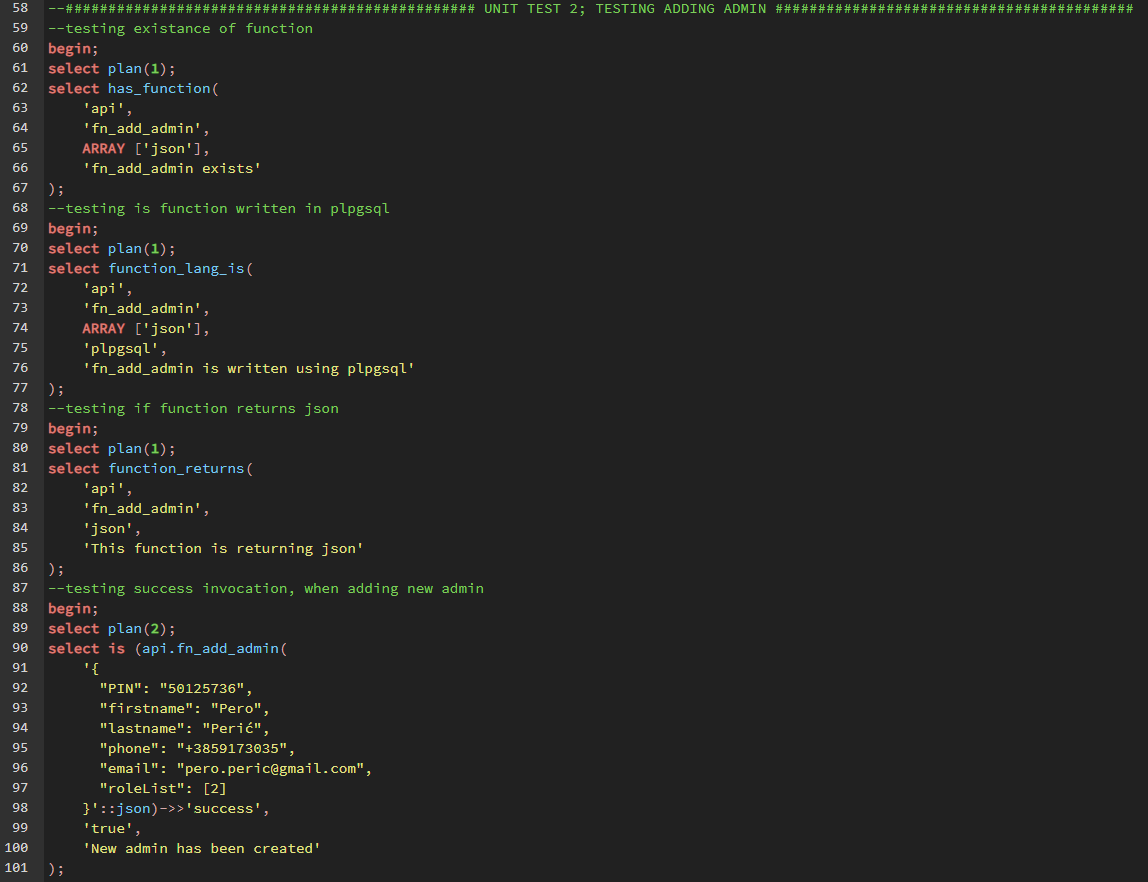
\includegraphics[width=\textwidth]{slike/unit_tests/ut_2/code_part1.png}
					\label{fig: IS2-code part 1}
				\end{figure}
				\begin{figure}[H]
					\centering
					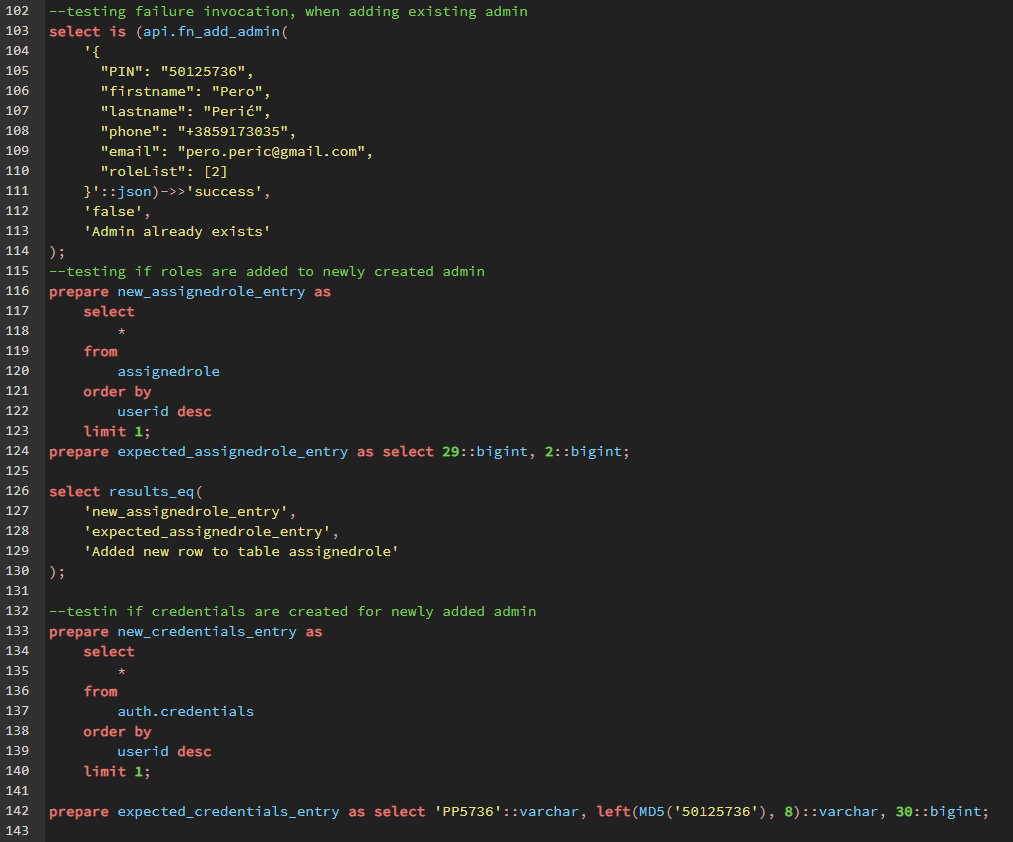
\includegraphics[width=\textwidth]{slike/unit_tests/ut_2/code_part2.png}
					\label{fig: IS2-code part 2}
				\end{figure}
				\begin{figure}[H]
					\centering
					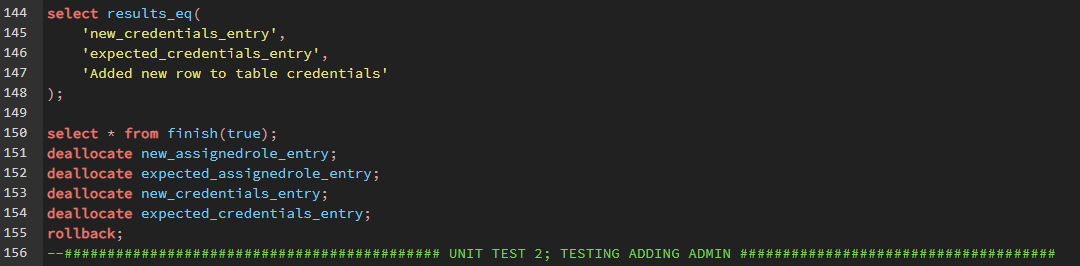
\includegraphics[width=\textwidth]{slike/unit_tests/ut_2/code_part3.png}
					\caption{Kod ispitnog slučaja 2}
					\label{fig: IS2-code part 3}
				\end{figure}
				\eject
				\subsection{Ispitni slučaj 3 - funkcionalnost brisanja administratora}
				Ovaj ispitni slučaj ispituje funkcionalnost brisanja administratora. Testovi ispitnog slučaja testiraju postoji li funkcija u bazi, je li funkcija napisana plpgsql jezikom te koji su ulazni i izlazni tipovi podataka funkcije. To se testira koristeći ugrađene funkcije pgTAP-a kao što su \textit{\texttt{has\_function}} za testiranje postoji li definirana funkcija u bazi, \textit{\texttt{function\_lang\_is}} za testiranje je li funkcija napisana plpgsql jezikom, \textit{\texttt{function\_returns}} za testiranje vraća li funkcija neki tip podataka ili je tipa void, \textit{\texttt{is\(\)}} ze provjeru dvaju argumenata te na osnovu njihovog podudaranje ili odudaranja se izbacuje rezultat. Rezultat je uvijek u obliku jednog reda sa jednom kolonom koja može sadržavati tekst \textit{ok $<$broj testa$>$ - $<$opis testa$>$} ili \textit{not ok $<$broj testa$>$ - $<$opis testa$>$}.
				\begin{figure}[H]
					\centering
					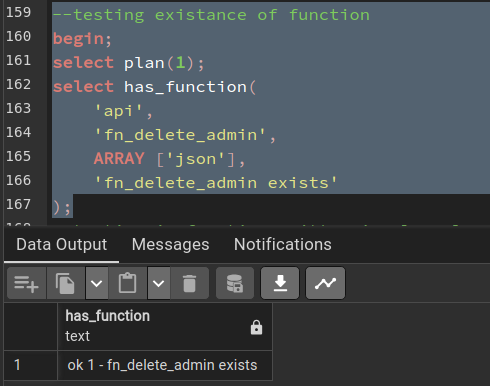
\includegraphics[width=\textwidth]{slike/unit_tests/ut_3/has_func.png}
					\caption{Pokretanje testa za provjeru postojanja funkcije}
					\label{fig: IS3-has_function}
				\end{figure}
				\begin{figure}[H]
					\centering
					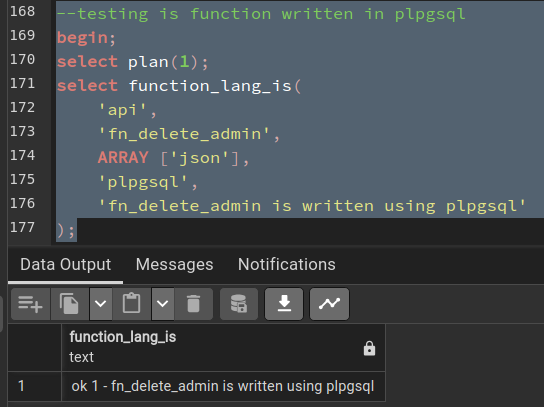
\includegraphics[width=\textwidth]{slike/unit_tests/ut_3/func_lang.png}
					\caption{Pokretanje testa za provjeru jezika kojim je napisana funkcija}
					\label{fig: IS3-function_lang}
				\end{figure}
				\begin{figure}[H]
					\centering
					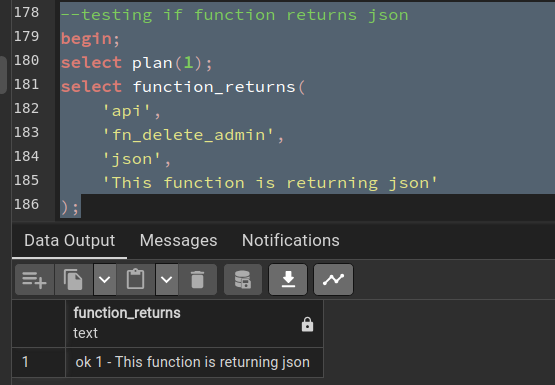
\includegraphics[width=\textwidth]{slike/unit_tests/ut_3/func_return.png}
					\caption{Pokretanje testa za provjeru povratnog tipa podatka funkcije}
					\label{fig: IS3-function_return}
				\end{figure}
				\begin{figure}[H]
					\centering
					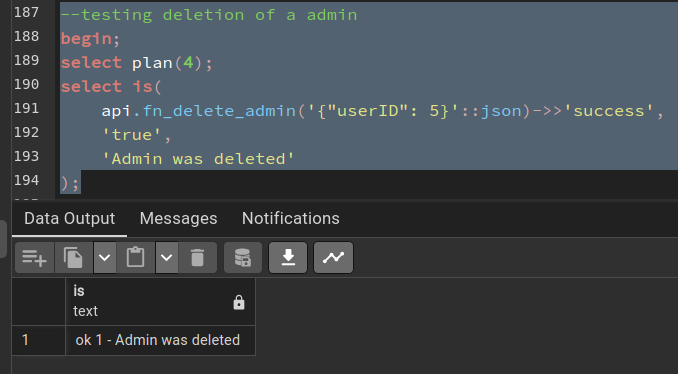
\includegraphics[width=\textwidth]{slike/unit_tests/ut_3/success_invocation.png}
					\caption{Pokretanje testa za provjeru rada same funkcije, uspjeh}
					\label{fig: IS3-uspješno izbrisan administrator}
				\end{figure}
				\begin{figure}[H]
					\centering
					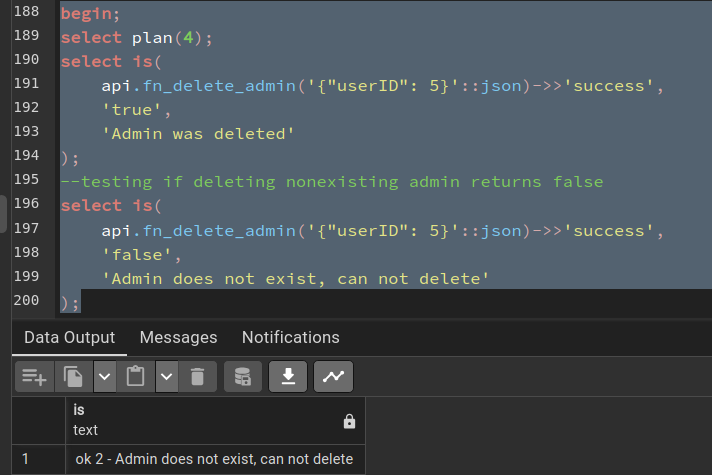
\includegraphics[width=\textwidth]{slike/unit_tests/ut_3/failure_invocation.png}
					\caption{Pokretanje testa za provjeru rada same funkcije, neuspjeh}
					\label{fig: IS3-administrator je već izbrisan ili ne postoji}
				\end{figure}
				\begin{figure}[H]
					\centering
					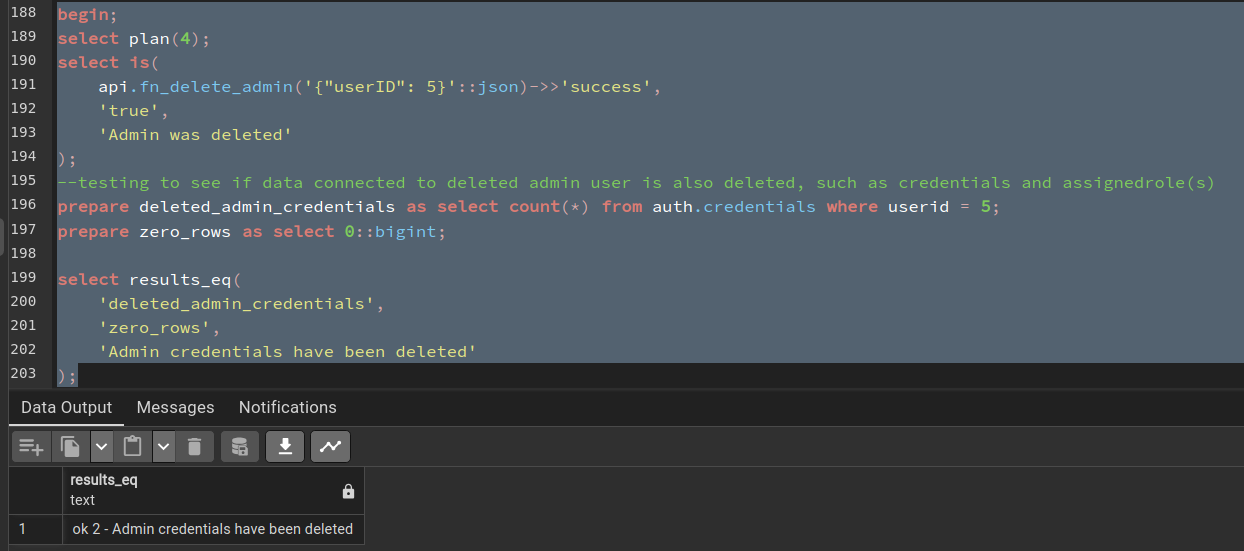
\includegraphics[width=\textwidth]{slike/unit_tests/ut_3/credentials_deletion.png}
					\caption{Pokretanje testa za provjeru automatskog brisanja vjerodajnica za izbrisanog administratora}
					\label{fig: IS3-brisanje vjerodajnice za obrisanog administratora}
				\end{figure}
				\begin{figure}[H]
					\centering
					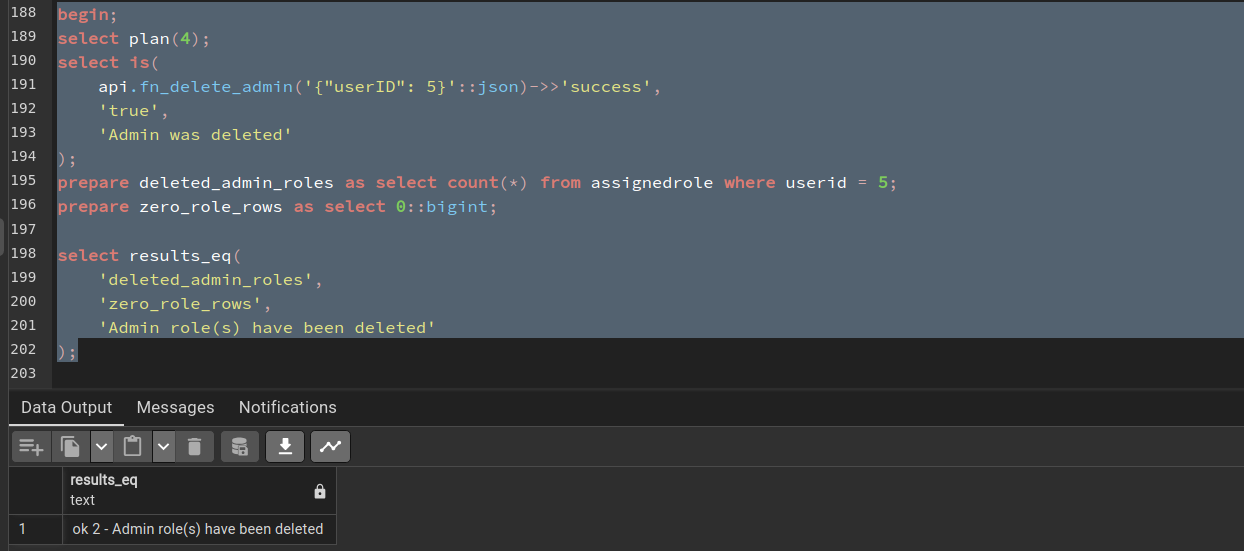
\includegraphics[width=\textwidth]{slike/unit_tests/ut_3/role_deletion.png}
					\caption{Pokretanje testa za provjeru automatskog brisanja pridjeljenih uloga za obrisanog administratora}
					\label{fig: IS3-brisanje pridjeljenih uloga za obrisanog administratora}
				\end{figure}
				\begin{figure}[H]
					\centering
					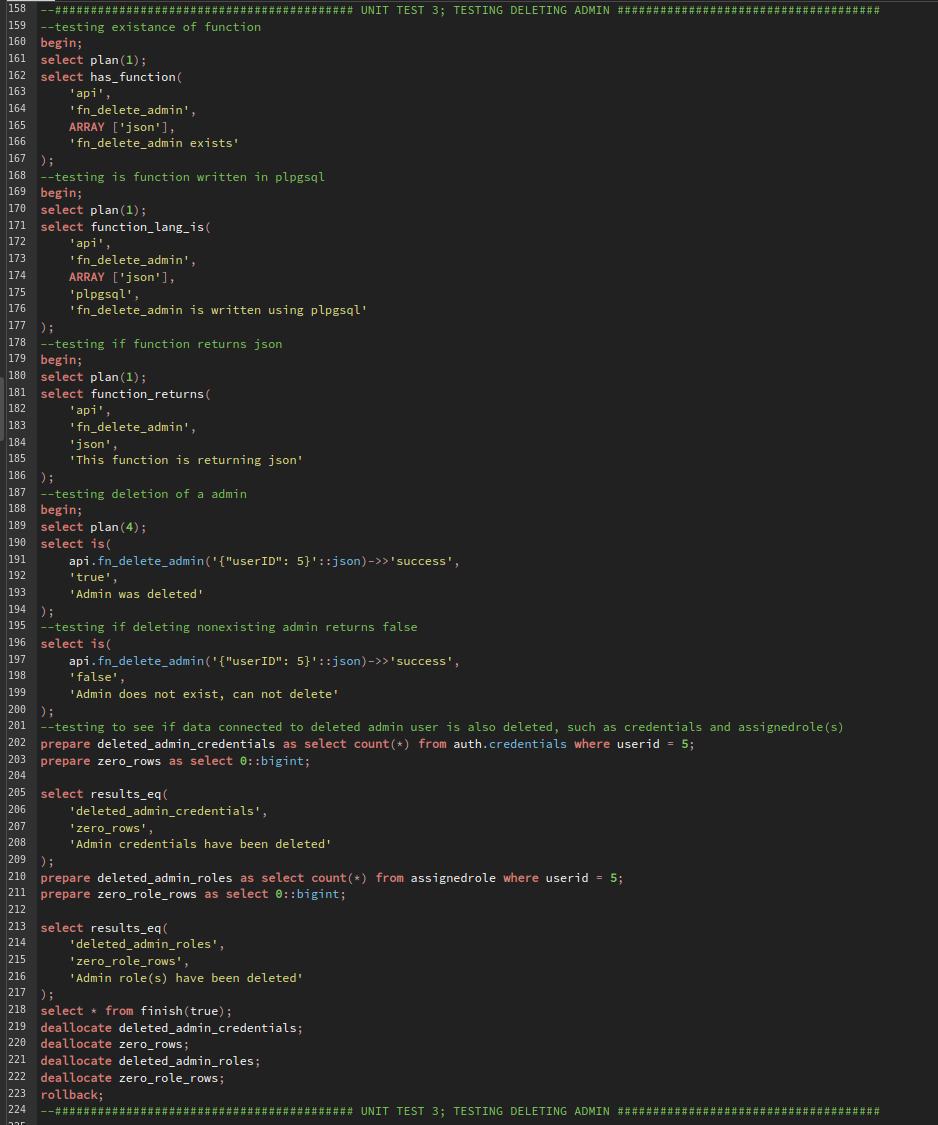
\includegraphics[width=\textwidth]{slike/unit_tests/ut_3/code.png}
					\caption{Kod ispitnog slučaja 3}
					\label{fig: IS3-kod}
				\end{figure}
				\eject
				\subsection{Ispitni slučaj 4 - funkcionalnost dodavanja smještaja}
				Ovaj ispitni slučaj ispituje funkcionalnost dodavanja smještaja. Testovi ispitnog slučaja testiraju postoji li funkcija u bazi, je li funkcija napisana plpgsql jezikom te koji su ulazni i izlazni tipovi podataka funkcije. To se testira koristeći ugrađene funkcije pgTAP-a kao što su \textit{\texttt{has\_function}} za testiranje postoji li definirana funkcija u bazi, \textit{\texttt{function\_lang\_is}} za testiranje je li funkcija napisana plpgsql jezikom, \textit{\texttt{function\_returns}} za testiranje vraća li funkcija neki tip podataka ili je tipa void, \textit{\texttt{is\(\)}} ze provjeru dvaju argumenata te na osnovu njihovog podudaranje ili odudaranja se izbacuje rezultat. Rezultat je uvijek u obliku jednog reda sa jednom kolonom koja može sadržavati tekst \textit{ok $<$broj testa$>$ - $<$opis testa$>$} ili \textit{not ok $<$broj testa$>$ - $<$opis testa$>$}.
				\begin{figure}[H]
					\centering
					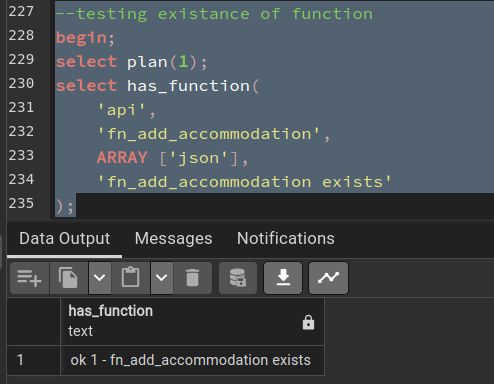
\includegraphics[width=\textwidth]{slike/unit_tests/ut_4/has_func.png}
					\caption{Pokretanje testa za provjeru postojanja funkcije}
					\label{fig: IS4-has_function}
				\end{figure}
				\begin{figure}[H]
					\centering
					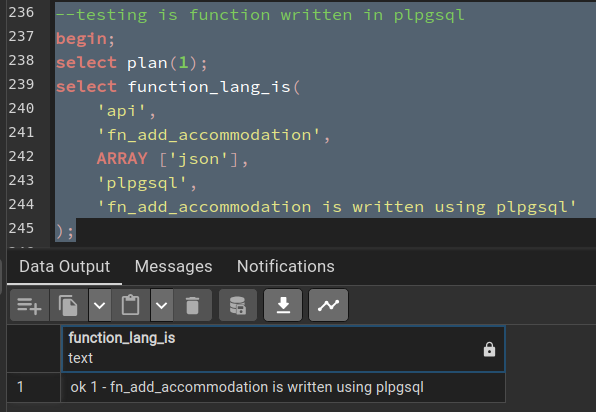
\includegraphics[width=\textwidth]{slike/unit_tests/ut_4/func_lang.png}
					\caption{Pokretanje testa za provjeru jezika kojim je napisana funkcija}
					\label{fig: IS4-function_lang}
				\end{figure}
				\begin{figure}[H]
					\centering
					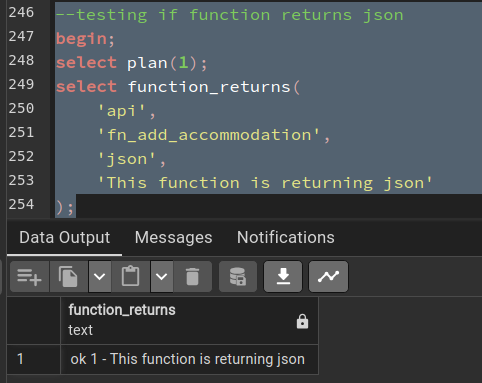
\includegraphics[width=\textwidth]{slike/unit_tests/ut_4/func_return.png}
					\caption{Pokretanje testa za provjeru povratnog tipa podatka funkcije}
					\label{fig: IS4-function_return}
				\end{figure}
				\begin{figure}[H]
					\centering
					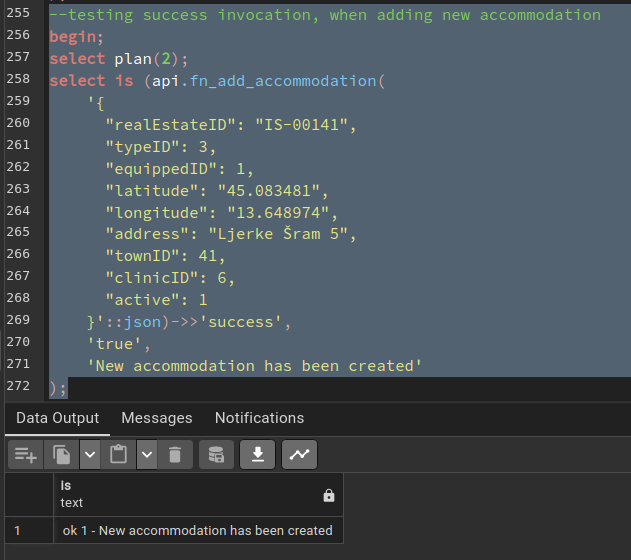
\includegraphics[width=\textwidth]{slike/unit_tests/ut_4/success_invocation.png}
					\caption{Pokretanje testa za provjeru rada same funkcije, uspjeh}
					\label{fig: IS4-uspješno kreiran smještaj}
				\end{figure}
				\begin{figure}[H]
					\centering
					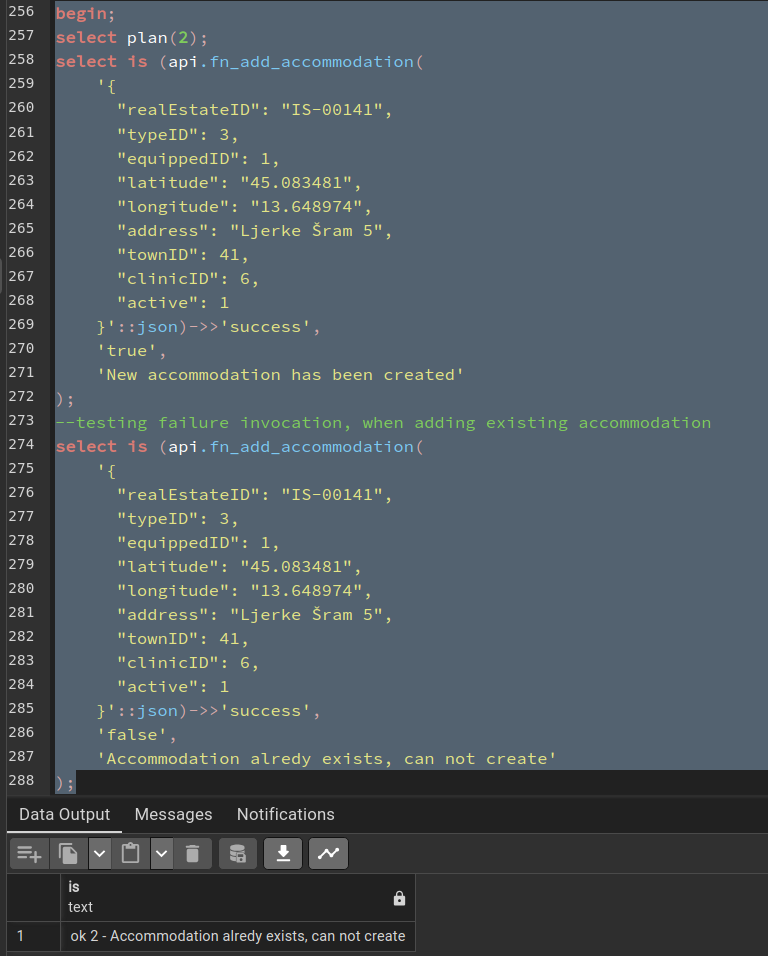
\includegraphics[width=\textwidth]{slike/unit_tests/ut_4/failure_invocation.png}
					\caption{Pokretanje testa za provjeru rada same funkcije, neuspjeh}
					\label{fig: IS4-smještaj nije kreiran, već postoji isti}
				\end{figure}
				\begin{figure}[H]
					\centering
					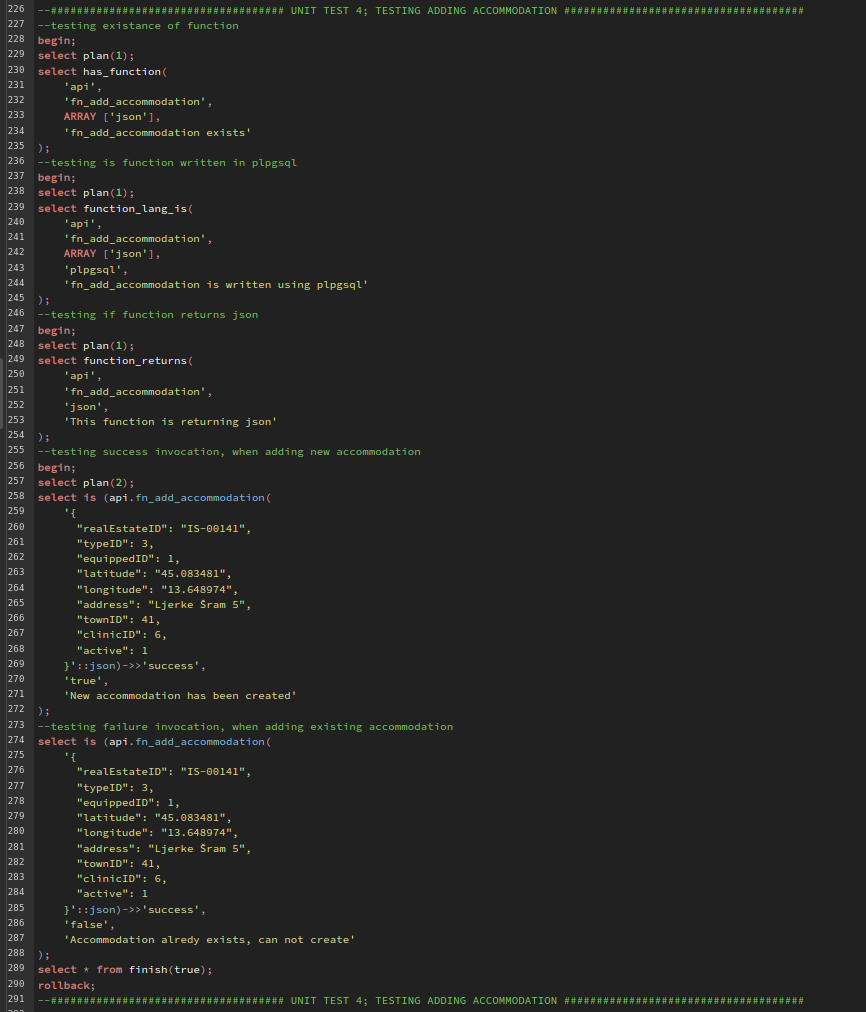
\includegraphics[width=\textwidth]{slike/unit_tests/ut_4/code.png}
					\caption{Kod ispitnog slučaja 4}
					\label{fig: IS4-kod}
				\end{figure}
				\eject
				\subsection{Ispitni slučaj 5 - funkcionalnost brisanja smještaja}
				Ovaj ispitni slučaj ispituje funkcionalnost brisanja smještaja. Testovi ispitnog slučaja testiraju postoji li funkcija u bazi, je li funkcija napisana plpgsql jezikom te koji su ulazni i izlazni tipovi podataka funkcije. To se testira koristeći ugrađene funkcije pgTAP-a kao što su \textit{\texttt{has\_function}} za testiranje postoji li definirana funkcija u bazi, \textit{\texttt{function\_lang\_is}} za testiranje je li funkcija napisana plpgsql jezikom, \textit{\texttt{function\_returns}} za testiranje vraća li funkcija neki tip podataka ili je tipa void, \textit{\texttt{is\(\)}} ze provjeru dvaju argumenata te na osnovu njihovog podudaranje ili odudaranja se izbacuje rezultat. Rezultat je uvijek u obliku jednog reda sa jednom kolonom koja može sadržavati tekst \textit{ok $<$broj testa$>$ - $<$opis testa$>$} ili \textit{not ok $<$broj testa$>$ - $<$opis testa$>$}.
				\begin{figure}[H]
					\centering
					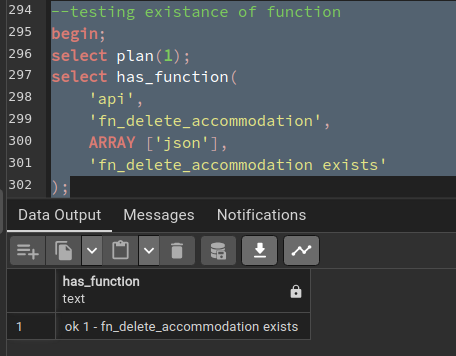
\includegraphics[width=\textwidth]{slike/unit_tests/ut_5/has_func.png}
					\caption{Pokretanje testa za provjeru postojanja funkcije}
					\label{fig: IS5-has_function}
				\end{figure}
				\begin{figure}[H]
					\centering
					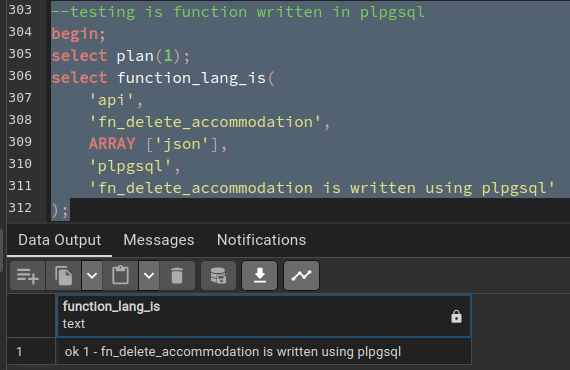
\includegraphics[width=\textwidth]{slike/unit_tests/ut_5/func_lang.png}
					\caption{Pokretanje testa za provjeru jezika kojim je napisana funkcija}
					\label{fig: IS5-function_lang}
				\end{figure}
				\begin{figure}[H]
					\centering
					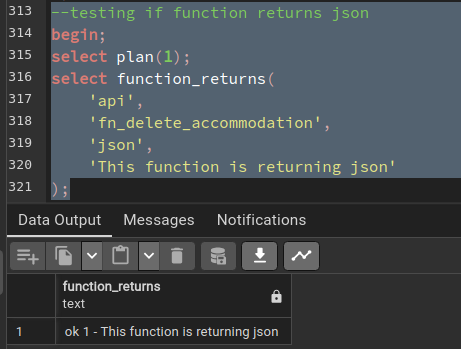
\includegraphics[width=\textwidth]{slike/unit_tests/ut_5/func_return.png}
					\caption{Pokretanje testa za provjeru povratnog tipa podatka funkcije}
					\label{fig: IS5-function_return}
				\end{figure}
				\begin{figure}[H]
					\centering
					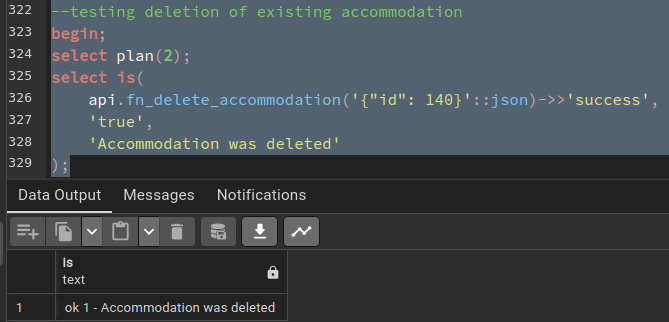
\includegraphics[width=\textwidth]{slike/unit_tests/ut_5/success_invocation.png}
					\caption{Pokretanje testa za provjeru rada same funkcije, uspjeh}
					\label{fig: IS5-uspješno izbrisan smještaj}
				\end{figure}
				\begin{figure}[H]
					\centering
					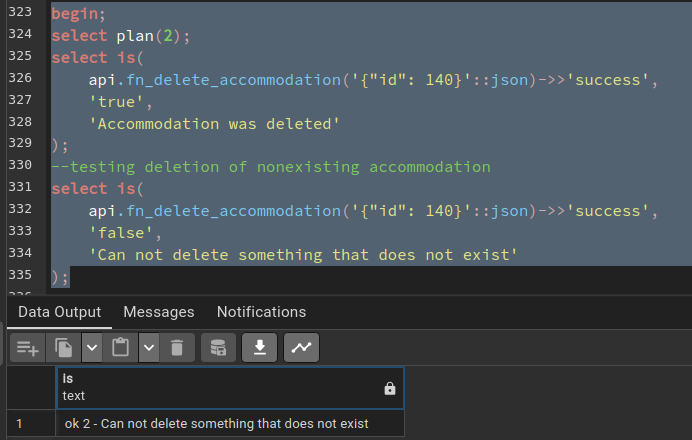
\includegraphics[width=\textwidth]{slike/unit_tests/ut_5/failure_invocation.png}
					\caption{Pokretanje testa za provjeru rada same funkcije, neuspjeh}
					\label{fig: IS5-smještaj je već izbrisan ili ne postoji}
				\end{figure}
				\begin{figure}[H]
					\centering
					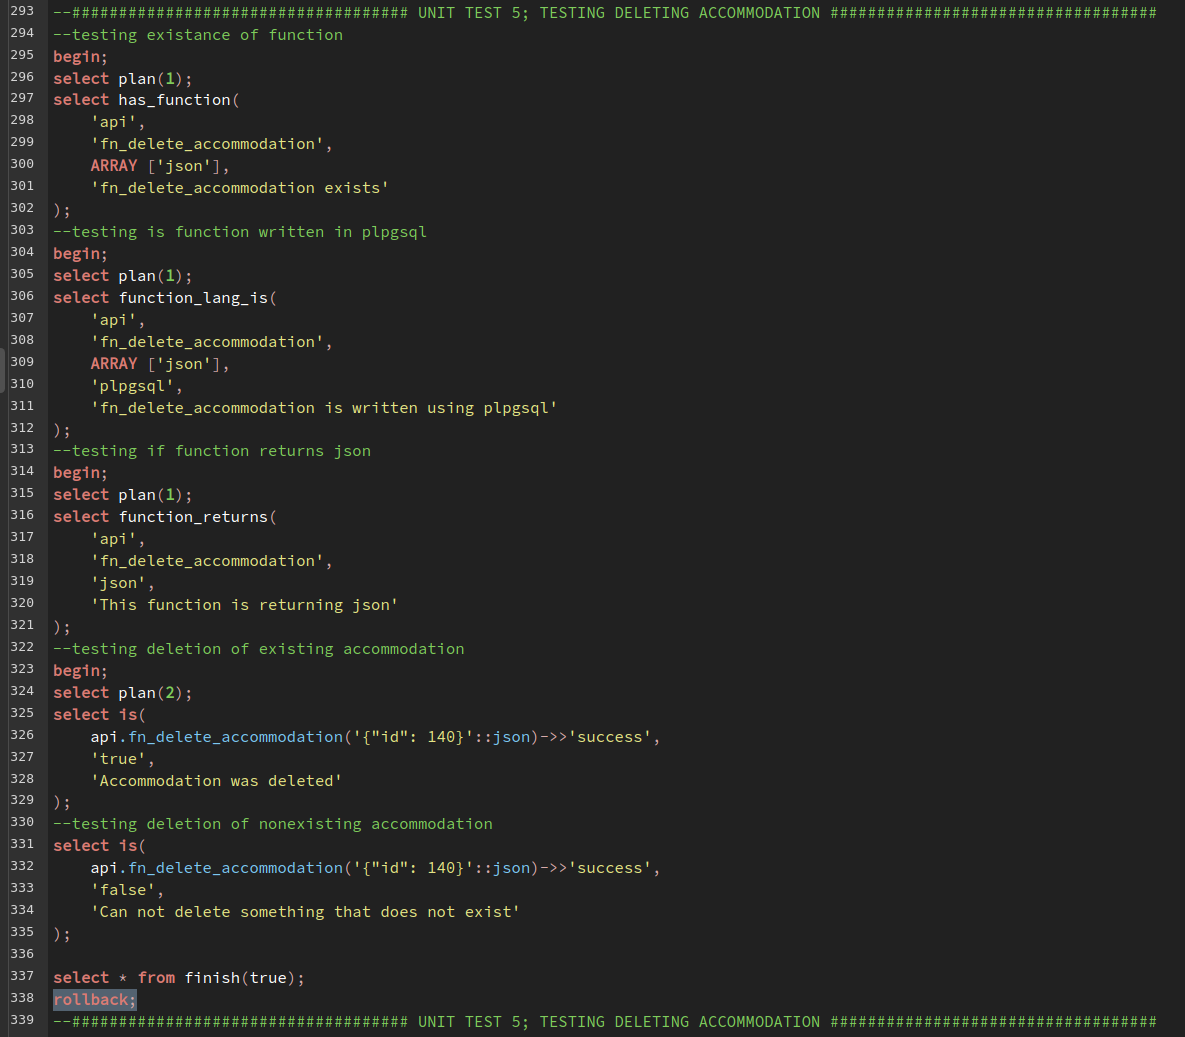
\includegraphics[width=\textwidth]{slike/unit_tests/ut_5/code.png}
					\caption{Kod ispitnog slučaja 5}
					\label{fig: IS5-kod}
				\end{figure}
				\eject
				\subsection{Ispitni slučaj 6 - funkcionalnost dohvaćanja posljednjeg unesenog realestateid-a}
				Ovaj ispitni slučaj ispituje funkcionalnost dohvaćanja posljednjeg unesenog realestateid-a. Testovi ispitnog slučaja testiraju postoji li funkcija u bazi, je li funkcija napisana plpgsql jezikom te koji su ulazni i izlazni tipovi podataka funkcije. To se testira koristeći ugrađene funkcije pgTAP-a kao što su \textit{\texttt{has\_function}} za testiranje postoji li definirana funkcija u bazi, \textit{\texttt{function\_lang\_is}} za testiranje je li funkcija napisana plpgsql jezikom, \textit{\texttt{function\_returns}} za testiranje vraća li funkcija neki tip podataka ili je tipa void, \textit{\texttt{is\(\)}} ze provjeru dvaju argumenata te na osnovu njihovog podudaranje ili odudaranja se izbacuje rezultat. Rezultat je uvijek u obliku jednog reda sa jednom kolonom koja može sadržavati tekst \textit{ok $<$broj testa$>$ - $<$opis testa$>$} ili \textit{not ok $<$broj testa$>$ - $<$opis testa$>$}.
				\begin{figure}[H]
					\centering
					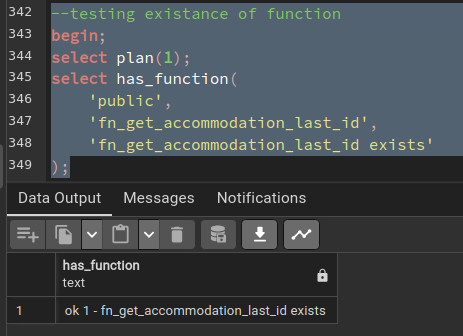
\includegraphics[width=\textwidth]{slike/unit_tests/ut_6/has_func.png}
					\caption{Pokretanje testa za provjeru postojanja funkcije}
					\label{fig: IS6-has_function}
				\end{figure}
				\begin{figure}[H]
					\centering
					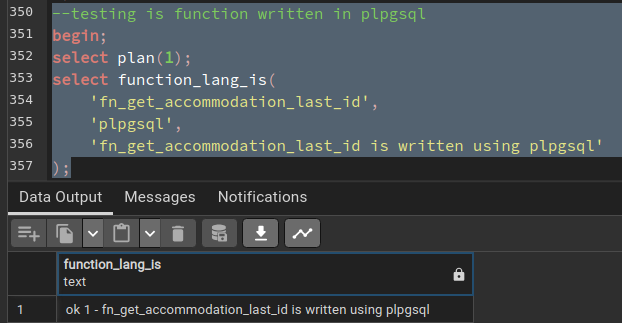
\includegraphics[width=\textwidth]{slike/unit_tests/ut_6/func_lang.png}
					\caption{Pokretanje testa za provjeru jezika kojim je napisana funkcija}
					\label{fig: IS6-function_lang}
				\end{figure}
				\begin{figure}[H]
					\centering
					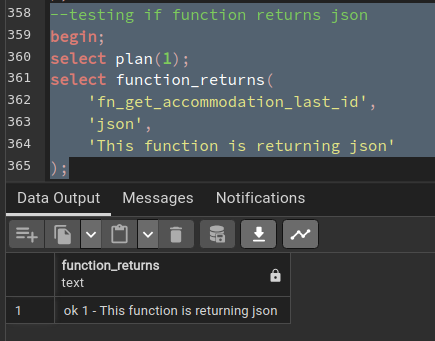
\includegraphics[width=\textwidth]{slike/unit_tests/ut_6/func_return.png}
					\caption{Pokretanje testa za provjeru povratnog tipa podatka funkcije}
					\label{fig: IS6-function_return}
				\end{figure}
				\begin{figure}[H]
					\centering
					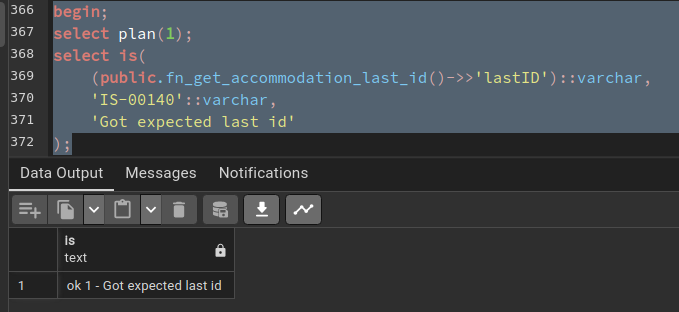
\includegraphics[width=\textwidth]{slike/unit_tests/ut_6/success_invocation.png}
					\caption{Pokretanje testa za provjeru rada same funkcije, uspjeh}
					\label{fig: IS6-uspješno dohvaćen posljednji realestateid}
				\end{figure}
				\begin{figure}[H]
					\centering
					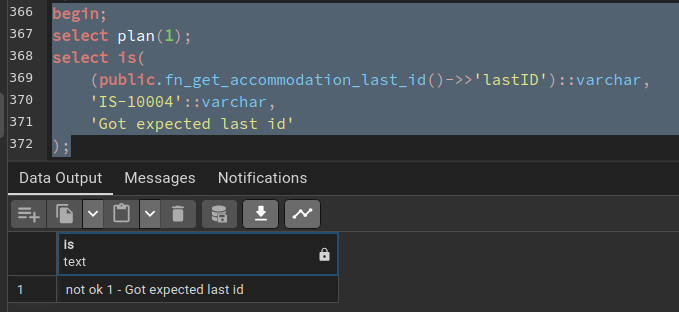
\includegraphics[width=\textwidth]{slike/unit_tests/ut_6/failure_invocation.png}
					\caption{Pokretanje testa za provjeru rada same funkcije, neuspjeh}
					\label{fig: IS6-navedeni realestateid ne postoji}
				\end{figure}
				\begin{figure}[H]
					\centering
					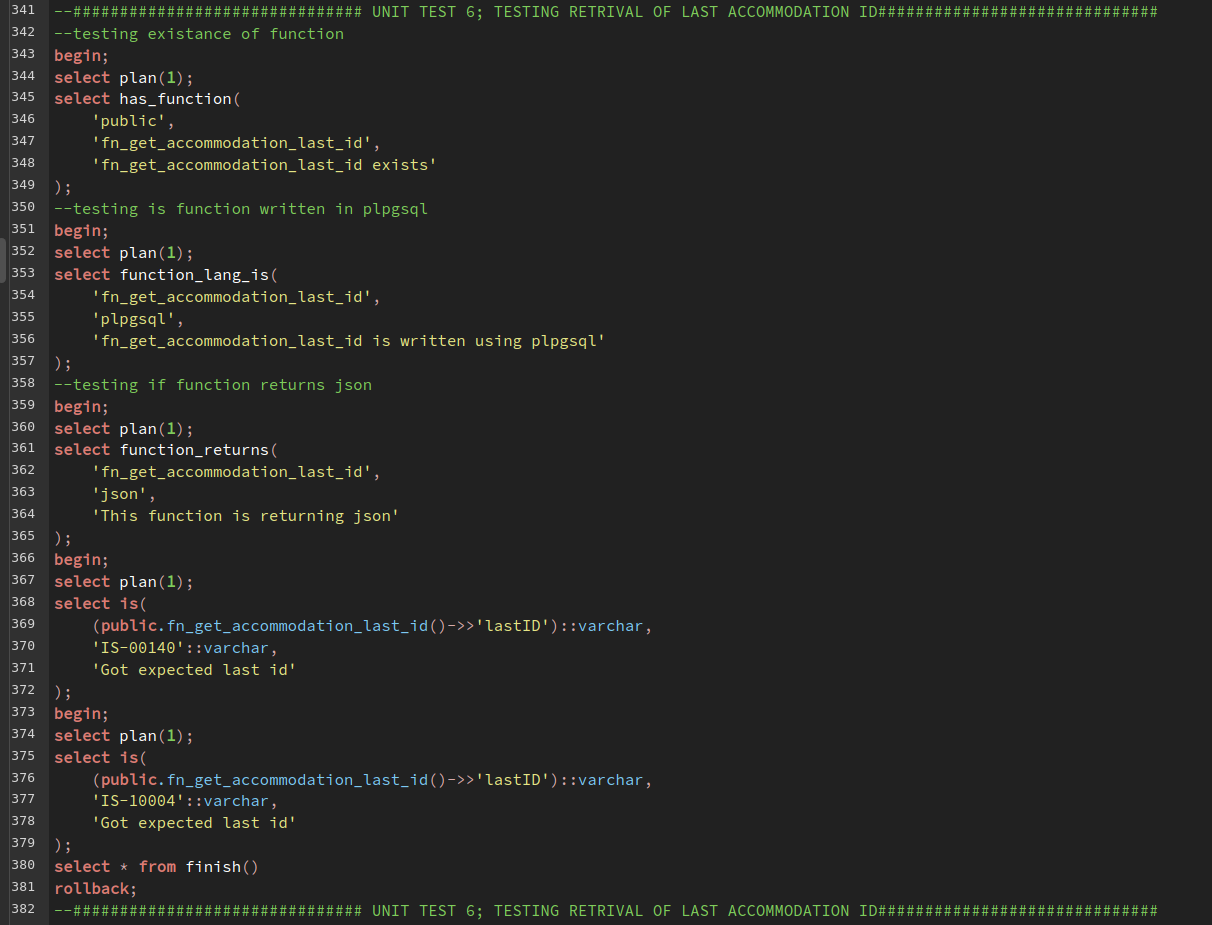
\includegraphics[width=\textwidth]{slike/unit_tests/ut_6/code.png}
					\caption{Kod ispitnog slučaja 6}
					\label{fig: IS6-kod}
				\end{figure}
				\eject
			\eject
			
			\subsection{Ispitivanje sustava}
			Ispitivanje sustava provedeno je s pomoću radnog okvira Selenium, konkretnije s pomoću dodatka za preglednik Selenium IDE. 
			\\U prvom ispitnom slučaju je ispitan slučaj dodavanja novog prijevoznika. Svi ulazni podaci su ispravni i očekivani izlaz je uspješno dodan prijevoznik.
			\begin{figure}[H]
				\centering
				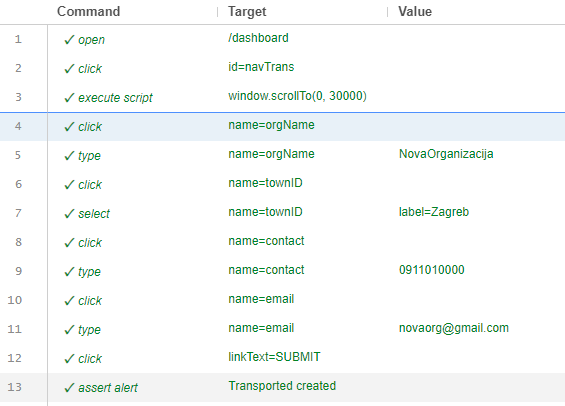
\includegraphics[width=\textwidth]{"slike/Selenium/transport testovi/registerTransportationGood_parameters.png"}
				\caption{Parametri prvog ispitnog slučaja}
				\label{fig: registerTransportationGood_parameters}
			\end{figure}
			\begin{figure}[H]
				\centering
				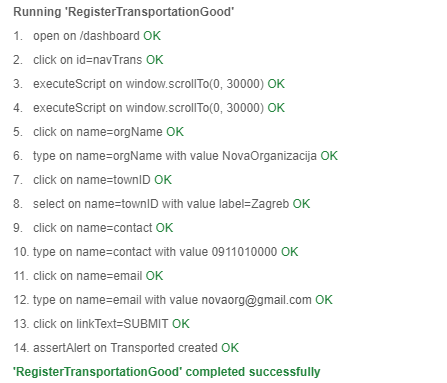
\includegraphics[width=\textwidth]{"slike/Selenium/transport testovi/registerTransportationGood_results.png"}
				\caption{Rezultat prvog ispitnog slučaja}
				\label{fig: registerTransportationGood_result}
			\end{figure}
			\eject
			U drugom ispitnom slučaju je ispitan slučaj dodavanja postojećeg prijevoznika. Svi ulazni podaci su ispravni (i identični kao u prethodnom ispitnom slučaju) te očekivani izlaz je neuspješno dodavanje prijevoznika jer ne može se dodati postojeći prijevoznik.
			\begin{figure}[H]
				\centering
				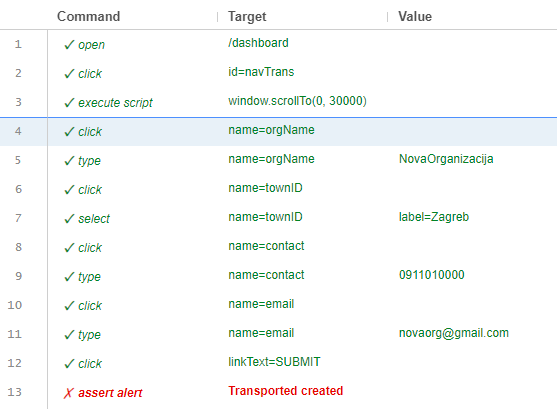
\includegraphics[width=\textwidth]{"slike/Selenium/transport testovi/registerTransportationAgain_parameters.png"}
				\caption{Parametri drugog ispitnog slučaja}
				\label{fig: registerTransportationAgain_parameters}
			\end{figure}
			\begin{figure}[H]
				\centering
				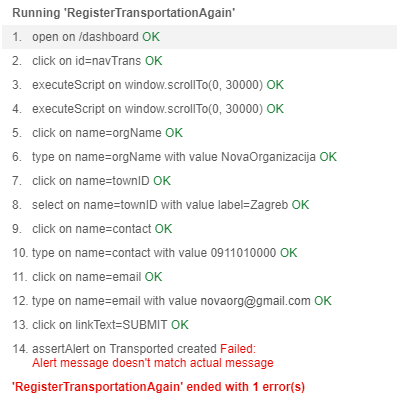
\includegraphics[width=\textwidth]{"slike/Selenium/transport testovi/registerTransportationAgain_results.png"}
				\caption{Rezultat drugog ispitnog slučaja}
				\label{fig: registerTransportationAgain_result}
			\end{figure}
			\eject
			U trećem ispitnom slučaju je ispitan slučaj dodavanja novog prijevoznika. Postoji jedan neispravan ulazni podatak (e-mail adresa je neispravna) te očekivani izlaz je neuspješno dodavanje prijevoznika jer svi ulazni podaci moraju biti ispravni kako bi se prijevoznik dodao.
			\begin{figure}[H]
				\centering
				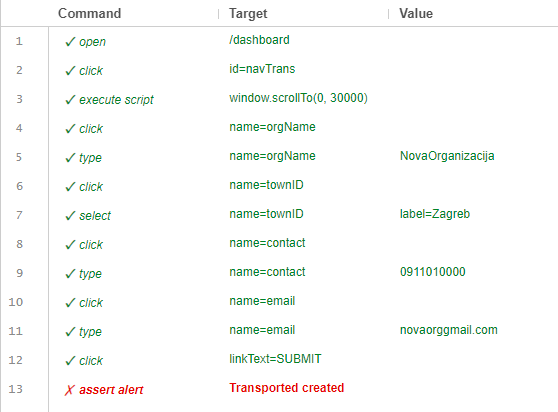
\includegraphics[width=\textwidth]{"slike/Selenium/transport testovi/registerTransportationBad_parameters.png"}
				\caption{Parametri trećeg ispitnog slučaja}
				\label{fig: registerTransportationBad_parameters}
			\end{figure}
			\begin{figure}[H]
				\centering
				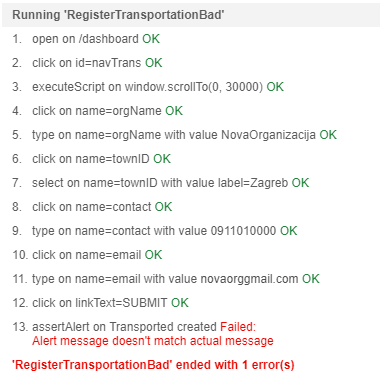
\includegraphics[width=\textwidth]{"slike/Selenium/transport testovi/registerTransportationBad_results.png"}
				\caption{Rezultat trećeg ispitnog slučaja}
				\label{fig: registerTransportationBad_result}
			\end{figure}
			\eject
			U četvrtom ispitnom slučaju je ispitan slučaj dodavanja novog vozila. Svi ulazni podaci su ispravni te očekivani izlaz je uspješno dodavanje vozila.
			\begin{figure}[H]
				\centering
				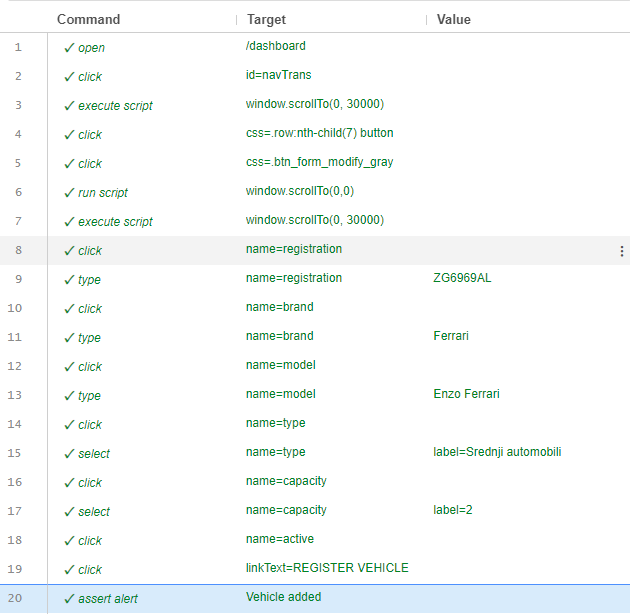
\includegraphics[width=\textwidth]{"slike/Selenium/transport testovi/addVehicleGood_parametri.png"}
				\caption{Parametri četvrtog ispitnog slučaja}
				\label{fig: addVehicleGood_parametri}
			\end{figure}
			\begin{figure}[H]
				\centering
				\includegraphics[width=\textwidth]{"slike/Selenium/transport testovi/addVehicleGood_rezultat.png"}
				\caption{Rezultat četvrtog ispitnog slučaja}
				\label{fig: addVehicleGood_rezultat}
			\end{figure}
			\eject
			U petom ispitnom slučaju je ispitan slučaj dodavanja postojećeg vozila. Svi ulazni podaci su ispravni (i identični kao u prethodnom ispitnom slučaju) te očekivani izlaz je neuspješno dodavanje vozila jer ne može se dodati postojeće vozilo.
			\begin{figure}[H]
				\centering
				\includegraphics[width=\textwidth]{"slike/Selenium/transport testovi/addVehicleAgain_parametri.png"}
				\caption{Parametri petog ispitnog slučaja}
				\label{fig: addVehicleAgain_parametri}
			\end{figure}
			\begin{figure}[H]
				\centering
				\includegraphics[width=\textwidth]{"slike/Selenium/transport testovi/addVehicleAgain_rezultat.png"}
				\caption{Rezultat petog ispitnog slučaja}
				\label{fig: addVehicleAgain_rezultat}
			\end{figure}
			\eject
			U šestom ispitnom slučaju je ispitan slučaj dodavanja novog vozila. Postoji jedan neispravan ulazni podatak (registracija je neispravna) te očekivani izlaz je neuspješno dodavanje vozila jer svi ulazni podaci moraju biti ispravni kako bi se vozilo dodalo.
			\begin{figure}[H]
				\centering
				\includegraphics[width=\textwidth]{"slike/Selenium/transport testovi/addVehicleBad_parametri.png"}
				\caption{Parametri šestog ispitnog slučaja}
				\label{fig: addVehicleBad_parametri}
			\end{figure}
			\begin{figure}[H]
				\centering
				\includegraphics[width=\textwidth]{"slike/Selenium/transport testovi/addVehicleBad_rezultat.png"}
				\caption{Rezultat šestog ispitnog slučaja}
				\label{fig: addVehicleBad_rezultat}
			\end{figure}
			\eject
			U sedmom ispitnom slučaju je ispitan slučaj dodavanja novog pacijenta. Svi ulazni podaci su ispravni te očekivani izlaz je uspješno dodavanje pacijenta.
			\begin{figure}[H]
				\centering
				\includegraphics[width=\textwidth]{"slike/Selenium/pacijent testovi/registerPatientGood_parameters.png"}
				\caption{Parametri sedmog ispitnog slučaja}
				\label{fig: registerPatientGood_parameters}
			\end{figure}
			\begin{figure}[H]
				\centering
				\includegraphics[width=\textwidth]{"slike/Selenium/pacijent testovi/registerPatientGood_results0.png"}
				\includegraphics[width=\textwidth]{"slike/Selenium/pacijent testovi/registerPatientGood_results1.png"}
				\caption{Rezultat sedmog ispitnog slučaja}
				\label{fig: registerPatientGood_results}
			\end{figure}
			\eject
			U osmom ispitnom slučaju je ispitan slučaj dodavanja postojećeg pacijenta. Svi ulazni podaci su ispravni (i identični kao u prethodnom ispitnom slučaju) te očekivani izlaz je neuspješno dodavanje pacijenta jer ne može se dodati postojeći pacijent.
			\begin{figure}[H]
				\centering
				\includegraphics[width=\textwidth]{"slike/Selenium/pacijent testovi/registerPatientAgain_parameters.png"}
				\caption{Parametri osmog ispitnog slučaja}
				\label{fig: registerPatientAgain_parameters}
			\end{figure}
			\begin{figure}[H]
				\centering
				\includegraphics[width=\textwidth]{"slike/Selenium/pacijent testovi/registerPatientAgain_results0.png"}
				\includegraphics[width=\textwidth]{"slike/Selenium/pacijent testovi/registerPatientAgain_results1.png"}
				\caption{Rezultat osmog ispitnog slučaja}
				\label{fig: registerPatientAgain_results}
			\end{figure}
			\eject
			U devetom ispitnom slučaju je ispitan slučaj dodavanja novog pacijenta. Postoji jedan neispravan ulazni podatak (e-mail adresa je neispravna) te očekivani izlaz je neuspješno dodavanje pacijenta jer svi ulazni podaci moraju biti ispravni kako bi se pacijent dodao.
			\begin{figure}[H]
				\centering
				\includegraphics[width=\textwidth]{"slike/Selenium/pacijent testovi/registerPatientBad_parameters.png"}
				\caption{Parametri devetog ispitnog slučaja}
				\label{fig: registerPatientBad_parameters}
			\end{figure}
			\begin{figure}[H]
				\centering
				\includegraphics[width=\textwidth]{"slike/Selenium/pacijent testovi/registerPatientBad_results0.png"}
				\includegraphics[width=\textwidth]{"slike/Selenium/pacijent testovi/registerPatientBad_results1.png"}
				\caption{Rezultat devetog ispitnog slučaja}
				\label{fig: registerPatientBad_results}
			\end{figure}
			\eject
			
		\section{Dijagram razmještaja}
			
			Na slici 5.42 prikazan je dijagram razmještaja. Sustav je baziran na arhitekturi “klijent-poslužitelj”. Korisnički pristup aplikaciji odvija se preko web preglednika. Na platformi Render smješteni su poslužitelji za frontend i middleware te baza podataka koja služi kao backend. Preko HTTP protokola ostvarena je komunikacija između korisnika i poslužitelja za frontend, te poslužitelja za frontend i poslužitelja za backend.
			
			\begin{figure}[H]
				\centering
				\includegraphics[width=\textwidth]{slike/UML_Deployment.png} %veličina slike u odnosu na originalnu datoteku i pozicija slike
				\caption{Dijagram razmještaja}
				\label{fig:dijagram razmještaja}
			\end{figure}
			
			\eject 
		
		\section{Upute za puštanje u pogon}
		
			Aplikacija je puštena u pogon na cloud servisu Render čime smo omogućili javni pristup aplikaciji. Render nudi brojne planove i mogućnosti, ali također nudi i besplatni plan za pokretanje malih testnih aplikacija. Za besplatni plan ne postoji mogućnost odabira virtualnog računala na kojem će se vrtiti aplikacije, baza i bilo što što se pusti u pogon. S tom informacijom nama kao krajnjem korisniku nije poznato na kojoj se mašini vrti, samo znamo da raspolažemo s 1 GiB prostora za pohranu baze podataka te RAM-om od 256 MB i CPU 100m. Sve potrebno za pokretanje instanci baze podataka ili drugih aplikacija je dostupno i podržani su brojni razvojni okviri i jezici.
			
			\break
			
			\textbf{\textit{Konfiguracija frontenda}}
			
				Za pokretanje frontend-a potrebno je odabrati opciju pokretanja web servisa na Render-u.
				\begin{figure}[H]
					\centering
					\includegraphics[width=\textwidth]{slike/render_web_service.png}
					\caption{Odabir opcije pokretanja instance web servisa}
					\label{fig: Render web service instance front}
				\end{figure}
				Zatim popunjavamo polja obaveznih podataka kao što su ime servisa, regija, grana repozitorija sa koje će se preuzeti kod, Runtime koji je u našem slučaju Node te "Build Command" gdje smo odabrali yarn. Poslije toga odabiremo besplatnu opciju instance te kreiramo web servis.
				\begin{figure}[H]
					\centering
					\includegraphics[width=\textwidth]{slike/create_web_service_part1.png}
					\label{fig: Render create web service part 1 front}
				\end{figure}
				\begin{figure}[H]
					\centering
					\includegraphics[width=\textwidth]{slike/create_web_service_part2.png}
					\caption{Popunjavanje forme za kreiranje instance web servisa}
					\label{fig: Render create web service part 2 front}
				\end{figure}
				
			\textbf{\textit{Konfiguracija baze/backenda}}
			
				Kako je cijeli backend napisan unutar same baze, u našem je slučaju samo bilo potrebno na Renderu pokrenuti instancu baze podataka. 
				\begin{figure}[H]
					\centering
					\includegraphics[width=\textwidth]{slike/render_new_instance.png}
					\caption{Odabir opcije pokretanja instance baze podataka}
					\label{fig: Render new instance}
				\end{figure}
				Naša baza podataka je PostgreSQL verzija 15 te još neke od mogućih opcija su odabir regije, za koju smo odabrali Frankfurt pošto je to najbliže. Može se specificirati i korisnik baze. Nakon što su obavezni podaci uneseni, klikom na gumb "Create Database" pokreće se postupak instanciranja baze i nedugo nakon toga su omogućene konekcije prema bazi. Onda se bilo kojim alatom, u našem slučaju PgAdmin4, može spojiti na bazu i početi s radom.
				\begin{figure}[H]
					\centering
					\includegraphics[width=\textwidth]{slike/create_db_form.png}
					\caption{Popunjavanje forme za kreiranje instance baze podataka}
					\label{fig: Render create new DB}
				\end{figure}
				Nadalje, kako bi se osigurala komunikacija između backenda i frontenda bilo je potrebno napraviti API koji će primati zahtjeve i prosljeđivati ih backendu. Za pokretanje API-ija potrebno je bilo odabrati opciju pokretanja web servisa(slika 5.42) koji se kasnije poveže sa GitHub repozitorijem te od tamo preuzmemo sav potreban kod.
				Nakon toga je potrebno unijeti obavezne podatke kao što su ime servisa, regija, grana repozitorija sa koje će se preuzeti kod te ono najvažnije, koji je "Runtime" našeg web servisa (slika 5.43). U našem slučaju smo odabrali Node, a za "Build Command" smo koristili yarn. Također se mogu dodati posebne Environmental variable koje omogućuju kontrolu verzije već instaliranog Node-a ili bilo kojeg drugog "Runtime-a". U slučaju Node-a najvažnije je da se u repozitoriju nalazi datoteka package.json koja omogućuje Render-u da preuzme sve potrebne biblioteke za pokretanje našeg API-ija.
				Na samome kraju kada se povuče kod sa repozitorija, moguće je pristupiti konzoli zaduženoj za upravljanje radom web servisa.
				\begin{figure}[H]
					\centering
					\includegraphics[width=\textwidth]{slike/render_deploy_status.png}
					\caption{Pristup konzoli za deploy}
					\label{fig: Render deploz console back}
				\end{figure}
			\eject 
